% File src/library/BGPhazard/vignettes/BGPhazard.Rnw
% Part of the R package, http://www.R-project.org
% Distributed under GPL 2 or later

\documentclass[letterpaper]{article}\usepackage[]{graphicx}\usepackage[]{color}
% maxwidth is the original width if it is less than linewidth
% otherwise use linewidth (to make sure the graphics do not exceed the margin)
\makeatletter
\def\maxwidth{ %
  \ifdim\Gin@nat@width>\linewidth
    \linewidth
  \else
    \Gin@nat@width
  \fi
}
\makeatother

\definecolor{fgcolor}{rgb}{0.345, 0.345, 0.345}
\newcommand{\hlnum}[1]{\textcolor[rgb]{0.686,0.059,0.569}{#1}}%
\newcommand{\hlstr}[1]{\textcolor[rgb]{0.192,0.494,0.8}{#1}}%
\newcommand{\hlcom}[1]{\textcolor[rgb]{0.678,0.584,0.686}{\textit{#1}}}%
\newcommand{\hlopt}[1]{\textcolor[rgb]{0,0,0}{#1}}%
\newcommand{\hlstd}[1]{\textcolor[rgb]{0.345,0.345,0.345}{#1}}%
\newcommand{\hlkwa}[1]{\textcolor[rgb]{0.161,0.373,0.58}{\textbf{#1}}}%
\newcommand{\hlkwb}[1]{\textcolor[rgb]{0.69,0.353,0.396}{#1}}%
\newcommand{\hlkwc}[1]{\textcolor[rgb]{0.333,0.667,0.333}{#1}}%
\newcommand{\hlkwd}[1]{\textcolor[rgb]{0.737,0.353,0.396}{\textbf{#1}}}%
\let\hlipl\hlkwb

\usepackage{framed}
\makeatletter
\newenvironment{kframe}{%
 \def\at@end@of@kframe{}%
 \ifinner\ifhmode%
  \def\at@end@of@kframe{\end{minipage}}%
  \begin{minipage}{\columnwidth}%
 \fi\fi%
 \def\FrameCommand##1{\hskip\@totalleftmargin \hskip-\fboxsep
 \colorbox{shadecolor}{##1}\hskip-\fboxsep
     % There is no \\@totalrightmargin, so:
     \hskip-\linewidth \hskip-\@totalleftmargin \hskip\columnwidth}%
 \MakeFramed {\advance\hsize-\width
   \@totalleftmargin\z@ \linewidth\hsize
   \@setminipage}}%
 {\par\unskip\endMakeFramed%
 \at@end@of@kframe}
\makeatother

\definecolor{shadecolor}{rgb}{.97, .97, .97}
\definecolor{messagecolor}{rgb}{0, 0, 0}
\definecolor{warningcolor}{rgb}{1, 0, 1}
\definecolor{errorcolor}{rgb}{1, 0, 0}
\newenvironment{knitrout}{}{} % an empty environment to be redefined in TeX

\usepackage{alltt}
\usepackage{Rd} 
\usepackage{caption}
\usepackage{subcaption}
\usepackage{amsmath}
\usepackage[OPTIONS]{hyperref}



%\VignetteIndexEntry{Introduction to BGPhazard}
\IfFileExists{upquote.sty}{\usepackage{upquote}}{}
\begin{document}
\title{Introduction to \code{BGPhazard}}
\author{Jos\'e A. Garc\'ia-Bueno and Luis E. Nieto-Barajas}
\maketitle

\section*{Abstract}

We present \code{BGPhazard}, an R package which computes hazard rates from a Bayesian nonparametric view. This is achieved by computing the posterior distribution of a gamma or a beta process through a Gibbs sampler. The purpose of this document is to guide the user on how to use the package rather than conducting a thorough analysis of the theoretical results. Nevertheless, section 2 briefly discuss the main results of the models proposed by Nieto-Barajas and Walker (2002) and by Nieto-Barajas (2003). These results will be helpful to understand the usage of the functions contained in the package. In section 3 we show some examples to illustrate the models.

\tableofcontents

\section{Introduction}

Survival analysis focuses on studying data related to the occurrence time of an event. A typical function is the \emph{survival function}, which in nonparametric statistics is estimated through the product limit estimator (Kaplan \& Meier, 1958). This estimator is used as an approximation to the survival function. In some cases, its stair-step nature can return misleading estimators in a neighborhood of the steps: just before and after each we will have significant differences between estimators.

Lack of smoothness on nonparametric estimations give rise to methods whose outputs are smooth functions. One of many approaches is given by Nieto-Barajas and Walker (2002) for the survival function. The theory behind these models combines Bayesian Statistics and Survival Analysis to obtain hazard rate estimates. Bayesian Statistics let us introduce previous knowledge to a data set to improve estimations. Nieto-Barajas \& Walker (2002) estimate the hazard function in segments by introducing dependence between each other so that information is shared and a smooth hazard rate is obtained. We review the three models contained in the package: beta model for discrete data, gamma model for continuous data and cox-gamma model for continuous data in a proportional hazards model.

A consequence of using a nonparametric Bayesian model with a dependence structure is that the resulting estimators are smoother than those obtained with a frequentist nonparametric model.

\section{Hazard rate estimation}

In this brief review, we examine a generalization of the independent gamma process of Walker and Mallick (1997) --gamma model--; then, a generalization of the beta process introduced by Hjort (1990) --beta model-- which is often used to model discrete failure times, and lastly, the proportional risk model extension to the gamma process that copes with explanatory variables that remain constant during time (Nieto-Barajas, 2003).

We provide nonparametric prior distributions for the hazard rate based on the dependence processes previously defined and we obtain the posterior distributions through a Bayesian update.

\subsection{Markov beta and gamma prior processes}

Let $\lambda_k$ represent the gamma process and let $\pi_k$ represent the beta process. Let $\theta_k$ represent both $\lambda_k$ and $\pi_k$. For interpretation of the Markov model, the main priority is to ensure
\begin{center}
$E[\theta_{k+1}|\theta_k]=a+b \theta_k $
\end{center}
where $(a,b)$ are fixed parameters and will typically depend on $k$. A latent process $\{u_k\}$ is introduced in order to obtain $\{\theta_k\}$ from
\begin{center}
  $\theta_1 \rightarrow u_1 \rightarrow \theta_2 \rightarrow u_2 \rightarrow \cdots$
\end{center}

\subsubsection*{Gamma Process}

Walker \& Mallick (1997) consider $\{\lambda_k\}$ as independent gamma variables, \emph{i.e.}, $\lambda_k \sim Ga(\alpha_k,\beta_k)$ independent for $k=1,2,...$ Nieto-Barajas \& Walker (2002) consider a dependent process for $\{\lambda_k\}$. They start with $\lambda_1\sim Ga(\alpha_1,\beta_1)$ and take $  u_k|\lambda_k \sim Po(c_k\lambda_k)$ and $\lambda_{k+1}|u_k \sim Ga(\alpha_{k+1} + u_k, \beta_{k+1} + c_k)$ and so on. These updates arise from the joint density
\begin{equation*}
  f(u,\lambda)=Ga(\lambda|\alpha,\beta)Po(u|c\lambda)
\end{equation*}
and so constitute a Gibbs type update. The difference is that they are changing the parameters $(\alpha,\beta,c)$ at each update so the chain is not stationary and marginally the $\{\lambda_k\}$ are not gamma.

However,
\begin{equation*}
  \mathrm{E}[\lambda_{k+1}|\lambda_k] = \frac{\alpha_{k+1}+c_k\lambda_k}{\beta_{k+1}+c_k}
\end{equation*}

If $c_k=0$, then $P(u_k=0)=1$ and hence the $\{\lambda_k\}$ are independent gamma and we have the prior process of Walker and Mallick (1997).

An important result is that if we take $\alpha_k=\alpha_1$ and $\beta_k=\beta_1$ to be constant for all $k$, then the process $\{u_k\}$ is a Poisson-gamma process with implied marginals $\lambda_k\sim Ga(\alpha_1,\beta_1)$. One can note that if $u_1$ is Poisson distributed and $\lambda_2|u_1$ is conditionally gamma, then $\lambda_2$ is never gamma.

\subsubsection*{Beta Process}

Nieto-Barajas and Walker (2002) start with $\pi_1 \sim Be(\alpha_1,\beta_1)$ and take $u_k|\pi_k \sim Bi(c_k,\pi_k)$, $\pi_{k+1}|u_k \sim Be(\alpha_{k+1} + u_k, \beta_{k+1} + c_k -u_k)$ and so on. These arise from a binomial-beta conjugate set-up, from the joint density
\begin{equation*}
  f(u,\pi)=Be(\pi|\alpha,\beta)Bi(u|c,\pi)
\end{equation*}
Clearly
\begin{equation*}
\mathrm{E}[\pi_{k+1}|\pi_k] = \frac{\alpha_{k+1}+c_k\pi_k}{\alpha_{k+1}+\beta_{k+1}+c_k}
\end{equation*}

As with the gamma process, if we choose $c_k=0$, then $P(u_k=0)=1$ and so the $\{u_k\}$ become independent beta and we obtain the prior of Hjort (1990). 

A significant result is that if we take $\alpha_k=\alpha_1$ and $\beta_k=\beta_1$ to be constant for all $k$, then the process $\{u_k\}$ is a binomial-beta process with marginals $u_k\sim BiBe(\alpha_1,\beta_1,c_k)$. Moreover, the process $\{\pi_k\}$ becomes strictly stationary and marginally $\pi_k\sim Be(\alpha_1,\beta_1)$.

\subsection{Prior to posterior analysis}

We use the gamma and beta processes to define nonparametric prior distributions. In order to obtain $f(\theta|data)$, we introduce the latent variable $u$ and so constitute a Gibbs update for $f(\theta|u,data)$ and $f(u|\theta,data)$. As we generate a sample from $f(\theta,u|data)$, we automatically obtain a sample from $f(\theta|data)$. Therefore, given $u$ from $f(u|\theta,data)$, we can obtain a sample from $f(\theta,u| data)$ by simulating from $\theta \sim f(\theta|u,data)$. 

It can be shown that
\begin{equation*}
f(\theta|u,data) \propto f(data|\theta)  \times f(\theta|u)
\end{equation*}
and
\begin{equation*}
 f(u|\theta,data) \propto f(data|\theta,u) \times f(u|\theta) \propto f(u|\theta)
\end{equation*}
because $u$ and $data$ are conditionally independent given $\theta$.

\subsubsection*{Gamma process}

Let $T$ be a continuous random variable with cumulative distribution function $F(t)=P(T\leq t)$ on $[0,\infty)$. Consider the time axis partition $0=\tau_0<\tau_1<\tau_2<\cdots$, and let $\lambda_k$ be the hazard rate in the interval $(\tau_{k-1},\tau_k]$, then the hazard function is given by 
\begin{equation*}
h (t) = \sum_{k=1}^{\infty} \lambda_kI_{(\tau_{k-1},\tau_k]}(t)
\end{equation*}

So, the cumulative distribution and density functions, given $\{ \lambda_k \}$, are $F(t|\{\lambda_k\}) = 1 - e^{-H(t)}$, $f(t|\{\lambda_k\}) = h(t) e^{-H(t)}$, where $H(t) = \int_0^t h(s)ds$. We also have that
\begin{equation*} 
f(\lambda_k|u_{k-1},u_k) = Ga(\alpha_{k} + u_{k-1} + u_k, \beta_{k} + c_{k-1} + c_k)
\end{equation*}

Therefore, given a sample $T_1,T_2,...,T_n$ from $f(t\{\lambda_k\})$, it is straightforward to derive
\begin{equation*} 
f(\lambda_k|u_{k-1},u_k,data) = Ga(\alpha_{k} + u_{k-1} + u_k + n_k, \beta_{k} + c_{k-1} + c_k + m_k),
\end{equation*}
where $n_k$ = number of uncensored observations in $(\tau_{k-1},\tau_k]$, $m_k = \sum_i r_{ki}$, and

\[ r_{ki} = \left \{
  \begin{array}{l l}
    \tau_k - \tau_{k-1}  & t_i > \tau_k  \\
    t_i - \tau_{k-1} & $t$ \in (\tau_{k-1},\tau_k] \\
    0 & $otherwise$
  \end{array} \right. \]

Additionally,

\begin{equation*}
P(u_k=u | \lambda_k,\lambda_{k+1},data) \propto f(u|\lambda) \propto \frac{[c_k(c_k+\beta_{k+1})\lambda_k\lambda_{k+1}]^u}{\Gamma(u+1)\Gamma(\alpha_{k+1}+u)}
\end{equation*}
with $u=0,1,2,...$. Hence, with these full conditional distributions, a Gibbs sampler is straightforward to implement in order to obtain posterior summaries.

We can learn about the $\{c_k\}$ by assigning an independent exponential distribution with mean $\epsilon$ for each $c_k$, $k=1,..,K-1$. The Gibbs sampler can be extended to include the full conditional densities for each $c_k$. It is not difficult to derive that a $c_k$ from $f(c_k|u,\lambda,data)$ can be taken from the density

\begin{equation*}
	f(c_k|u_k,\lambda_k,\lambda_{k+1}) \propto (\beta_{k+1}+c_k)^{\alpha_{k+1}+u_k}c_k^{u_k}\exp\left\{ -c_k \left (\lambda_{k+1}+\lambda_k+\frac{1}{\epsilon} \right) \right\}
\end{equation*}
for $c_k >0$.

Dependence between $c_k'$s can be introduced through a hierarchical model via assigning a distribution to $\epsilon \sim Ga(a_0,b_0)$. The update would be given by: 
\begin{equation*}
f(\epsilon|\{c_k\}) = Ga\left(\epsilon |a_0 + K, b_0 + \sum_{k=1}^K c_k \right)
\end{equation*}
where $K$ is the number of intervals generated by the time axis partition. This hierarchical specification of the initial distribution for $c_k$ let us assign a better value for $c_k$.

Simulating from this distribution is not so straightforward. However, we construct a hybrid algorithm using a Metropolis-Hastings scheme taking advantage of the Markov chain generated by the Gibbs sampling.

\subsubsection*{Beta process}

Let $T$ be a discrete random variable taking values in the set $\{\tau_1,\tau_2,...\}$ with probability density function $f(\tau_k)=P(T=\tau_k)$. Let $\pi_k$ be the hazard rate at $\tau_k$, then the cumulative distribution and the density functions, given $\{\pi_k\}$, are $F(\tau_j|\{\pi_k\}) = 1 - \prod_{k=1}^j(1-\pi_k)$ and $ f(\tau_j|\{\pi_k\}) = \pi_j \prod_{k=1}^{j-1}(1-\pi_k)$

The conditional distribution of $\pi_k$ is
\begin{equation*}
 f(\pi_k|u_{k-1},u_k) = Be(\pi_k|\alpha_k+ u_{k-1} + u_k,\beta_k + c_{k-1} -u_{k-1}+ c_k-u_k),
 \end{equation*}

Thus, given a sample $T_1,T_2,...,T_n$ form $f(\cdot|\{\pi_k\})$ it is straightforward to derive
 \begin{equation*}
 f(\pi_k | u_{k-1}, u_k, data) =Be(\pi_k|\alpha_k+ u_{k-1} + u_k +n_k,\beta_k + c_{k-1} -u_{k-1}+ c_k-u_k+m_k),
\end{equation*}
 where $n_k$ = number of failures at $\tau_k$, $m_k = \sum_i r_{ki}$ and
\[ r_{ki} = \left \{
  \begin{array}{l l}
    1 & \quad t_i > \tau_k  \\
    0 & \quad $otherwise$
  \end{array} \right. \]

Additionally,
\begin{equation*}
P(u_k=u | \pi_k,\pi_{k+1}, data) \propto \frac{\theta_k^u}{\Gamma(u+1)\Gamma(c_k-u+1)\Gamma(\alpha_{k+1}+u)\Gamma(\beta_{k+1}+c_k-u)}
\end{equation*}
with $u=0,1,...,c_k$ and
\begin{equation*}
\theta_k  = \frac{\pi_k\pi_{k+1}}{(1-\pi_k)(1-\pi_{k+1})}
\end{equation*}
As before, obtaining posterior summaries via Gibbs sampler is simple.

We can learn about the $\{c_k\}$ via assigning each $c_k$ an independent Poisson distribution with mean $\epsilon$. The Gibbs sampler can be extended to include the full conditional densities for each $c_k$. A $c_k$ from $f(c_k|u,\pi,data)$ can be taken from the density

\begin{equation*}
  f(c_k|u_k,\pi_k,\pi_{k+1}) \propto \frac{\Gamma(\alpha_{k+1}+\beta_{k+1}+c_k)}{\Gamma(\beta_{k+1}+c_k-u_k)\Gamma(c_k-u_k+1)} \left[\epsilon (1-\pi_{k+1})(1-\pi_k) \right]^{c_k}
\end{equation*}
with $c_k \in \{u_k,u_k+1,u_k+2,...\}$.

Dependence between $c_k$'s can be introduced through a hierarchical model via assigning a distribution to $\epsilon \sim Ga(a_0,b_0)$. So the update would be given by: 
\begin{equation*}
f(\epsilon|\{c_k\}) = Ga\left(\epsilon |a_0 + K, b_0 + \sum_{k=1}^K c_k \right)
\end{equation*}
where $K$ is the number of discrete values in random variable $T$.

\subsubsection*{Cox-gamma model}

Differing from most of the previous Bayesian analysis of the proportional hazards model, Nieto-Barajas (2003) models the baseline hazard rate function with a stochastic process. Let $T_i$ be a non negative random variable which represents the failure time of $i$ and $Z_i=(Z_{i1},...,Z_{ip})$ the vector containing its $p$ explanatory variables. Therefore, the hazard function for individual $i$ is:
\begin{equation*}
\lambda_i(t)=\lambda_0(t)exp\{Z_i'\theta\}
\end{equation*}
where $\lambda_0(t)$ is the baseline hazard rate and $\theta$ is regression's coefficient vector. The cumulative hazard function for individual $i$ becomes
\begin{equation*}
H_i(t)=\sum_{k=1}^{\infty}\lambda_k W_{i,k}(t,\lambda),
\end{equation*}
where,

\[ W_{i,k}(t,\theta) = \left \{
  \begin{array}{l l}
    (\tau_k - \tau_{k-1})\exp\{Z_i'\theta \} & t_i > \tau_k  \\
    (t_i - \tau_{k-1})\exp\{Z_i'\theta \} & t_i \in (\tau_{k-1},\tau_k]  \\
    0 & otherwise
  \end{array} \right. \]

Given a sample of possible right-censored observations where $T_1, ..., T_n$ are uncensored and $T_{n_u+1},...,T_n$ are right-censored, the conditional posterior distributions for the parameters of the semi-parametric model are:

\begin{itemize}
\item{$f(\lambda_k | u_{k-1}, u_k, data,\theta) = Ga(\lambda_k|\alpha_k+ u_{k-1} + u_k + n_k,\beta_k + c_{k-1} + c_k+m_k(\theta))$}
\item{$P(u_k=u | \lambda_k,\lambda_{k+1},data) \propto f(u|\lambda) \propto \frac{[c_k(c_k+\beta_{k+1})\lambda_k\lambda_{k+1}]^u}{\Gamma(u+1)\Gamma(\alpha_{k+1}+u)}$}
\item{$f(\theta|\lambda,data)\propto  f(\theta) \exp\left\{{\sum_{i=1}^{n_u} \theta'Z_i} -\sum_{k=1}^\infty \lambda_k m_k(\theta) \right\} $}
\end{itemize}
where $n_k=\sum_{i=1}^{n_u}I_{(\tau_{k-1},\tau_k]}(t_i)$ and $m_k(\theta)=\sum_{i=1}^n W_{i,k}(t_i,\theta)$.

Similarly as we pointed out in the previous two cases, we incorporate a hyper prior process for the $\{c_k\}$ such that $c_k\sim Ga(1,\epsilon_k)$. The set of full conditional posterior distributions can then be extended to include

\begin{equation*}
f(c_k|u_k,\lambda_k,\lambda_{k+1}) \propto (\beta_{k+1}+c_k)^{\alpha_{k+1}+u_k}c_k^{u_k}\exp\left\{ -c_k \left (\lambda_{k+1}+\lambda_k+\frac{1}{\epsilon} \right) \right\}
\end{equation*}

Dependence between $c_k$'s can be introduced through a hierarchical model via assigning a distribution to $\epsilon \sim Ga(a_0,b_0)$. So the update would be given by: 
\begin{equation*}
f(\epsilon|\{c_k\}) = Ga\left(\epsilon |a_0 + K, b_0 + \sum_{k=1}^K c_k \right)
\end{equation*}
where $K$ is the number of intervals generated by the time axis partition. This hierarchical specification of the initial distribution for $c_k$ let us assign a better value for $c_k$.

\section{Examples}

We present some of the examples contained in the documentation of the package to illustrate some of the effects of setting different parameters --how to define the partition or how $c_k$ vector is obtained--. First, we start showing examples for the Gamma model, then for the Beta model and finally for the Cox-Gamma model.

\subsection{Gamma model examples}

For this model, we will be using the control observations of the 6-MP data set (Freireich, E. J., et al., 1963) --data from a trial of 42 leukemia patients organised by pairs in which the first element of the pair is treated with a drug and the other is control--. For examples 1 to 4, we use a partition of unitary length intervals; for the last three examples --5, 6 \& 7--, we use uniformly-dense intervals. The \code{"time"} column is taken as the observed times vector --\code{times}-- and the \code{"cens"} column as the censoring status vector --\code{delta}--:

\begin{knitrout}
\definecolor{shadecolor}{rgb}{0.969, 0.969, 0.969}\color{fgcolor}\begin{kframe}
\begin{alltt}
\hlkwd{data}\hlstd{(gehan)}
\hlstd{times} \hlkwb{<-} \hlstd{gehan}\hlopt{$}\hlstd{time[gehan}\hlopt{$}\hlstd{treat} \hlopt{==} \hlstr{"6-MP"}\hlstd{]}
\hlstd{delta} \hlkwb{<-} \hlstd{gehan}\hlopt{$}\hlstd{cens[gehan}\hlopt{$}\hlstd{treat} \hlopt{==} \hlstr{"6-MP"}\hlstd{]}
\end{alltt}
\end{kframe}
\end{knitrout}

Now that we have a time and censoring status vector, we can run several examples for this model. Default values are used for each function unless otherwise noted. Every example shows our estimate overlapped with the Nelson-Aalen / Kaplan-Meier estimator, so the user can compare them.

\subsubsection{Example 1. Independence case. Unitary length intervals}

We obtain with our model the Nelson-Aalen and Kaplan-Meier estimators by defining $c_k$ as a null vector --through fixing \code{type.c = 1}--. A unitary partitioned axis is obtained by fixing \code{type.t = 2}. In Figure \ref{fig:G1} we show that our estimators --under independence-- return the same results as the Nelson-Aalen and Kaplan-Meier estimators.

\begin{knitrout}
\definecolor{shadecolor}{rgb}{0.969, 0.969, 0.969}\color{fgcolor}\begin{kframe}
\begin{alltt}
\hlstd{ExG1} \hlkwb{<-} \hlkwd{GaMRes}\hlstd{(times, delta,} \hlkwc{type.t} \hlstd{=} \hlnum{2}\hlstd{,} \hlkwc{K} \hlstd{=} \hlnum{35}\hlstd{,} \hlkwc{type.c} \hlstd{=} \hlnum{1}\hlstd{,}
               \hlkwc{iterations} \hlstd{=} \hlnum{3000}\hlstd{)}
\hlkwd{GaPloth}\hlstd{(ExG1,} \hlkwc{confint} \hlstd{=} \hlnum{FALSE}\hlstd{)}
\end{alltt}
\end{kframe}
\end{knitrout}
\begin{figure}
  \centering
  \begin{subfigure}[a]{\textwidth}\centering
    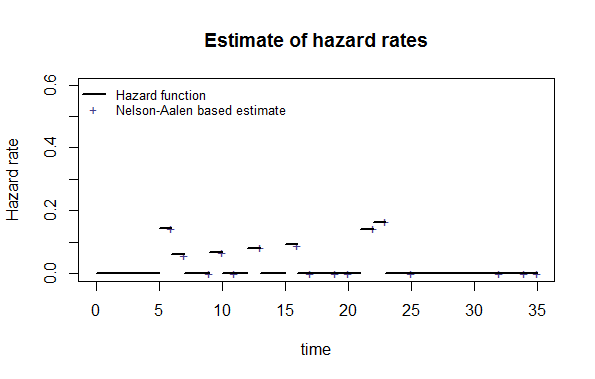
\includegraphics[width=\textwidth]{G11.png}
    \caption{Hazard rates}
  \end{subfigure}
  \begin{subfigure}[b]{\textwidth}\centering
    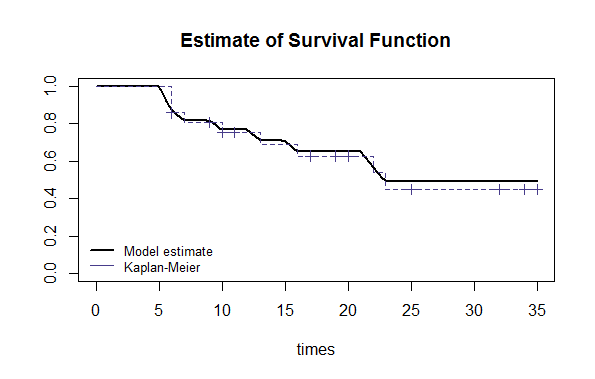
\includegraphics[width=\textwidth]{G12.png}
    \caption{Survival function}
  \end{subfigure}
  \caption{Gamma Example 1 - Independence case. Unitary length intervals}
  \label{fig:G1}
\end{figure}

\subsubsection{Example 2. Introducing dependence through c. Unitary length intervals}

The influence of $c$ --or \code{c.r}-- can be understood as a dependence parameter: the greater the value of each $c_k$, $k=0,1,2,...,K-1$, the higher the dependence between intervals $k$ and $k+1$. For this example, we assign a fixed value to vector $c$, so we use \code{type.c = 2}. Comparing with the previous example, we see that the estimates that were zero, now have a positive value --see Figures \ref{fig:G1} and \ref{fig:G2}--. Note  how this model compares to Example 5 --see Figure \ref{fig:G5}--. The difference between those examples is how the partition is defined.

\begin{knitrout}
\definecolor{shadecolor}{rgb}{0.969, 0.969, 0.969}\color{fgcolor}\begin{kframe}
\begin{alltt}
\hlstd{ExG2} \hlkwb{<-} \hlkwd{GaMRes}\hlstd{(times, delta,} \hlkwc{type.t} \hlstd{=} \hlnum{2}\hlstd{,} \hlkwc{K} \hlstd{=} \hlnum{35}\hlstd{,} \hlkwc{type.c} \hlstd{=} \hlnum{2}\hlstd{,}
               \hlkwc{c.r} \hlstd{=} \hlkwd{rep}\hlstd{(}\hlnum{50}\hlstd{,} \hlnum{34}\hlstd{),} \hlkwc{iterations} \hlstd{=} \hlnum{3000}\hlstd{)}
\hlkwd{GaPloth}\hlstd{(ExG2)}
\end{alltt}
\end{kframe}
\end{knitrout}

\begin{figure}
  \centering
  \begin{subfigure}[a]{\textwidth}\centering
    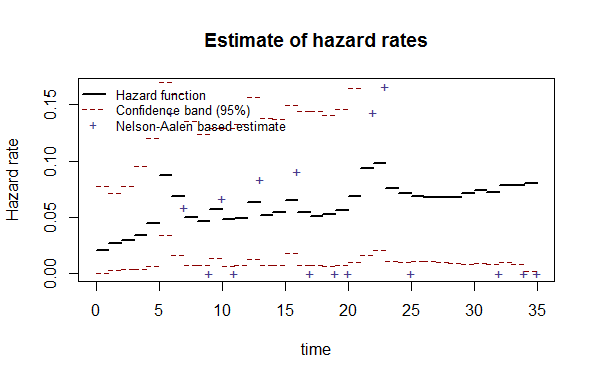
\includegraphics[width=\textwidth]{G21.png}
    \caption{Hazard rates}
  \end{subfigure}
  \begin{subfigure}[b]{\textwidth}\centering
    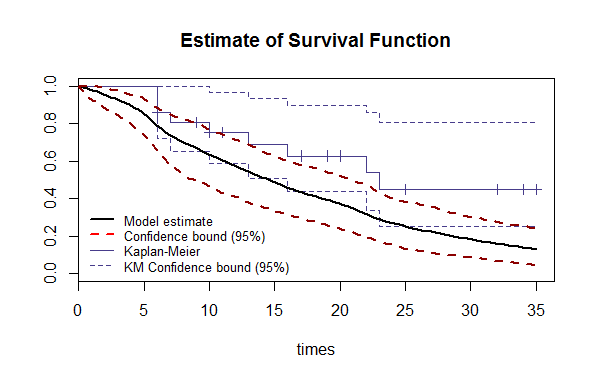
\includegraphics[width=\textwidth]{G22.png}
    \caption{Survival function}
  \end{subfigure}
  \caption{Gamma Example 2 - Introducing dependence through c ($c_k=50, \forall k$). Unitary length intervals}
  \label{fig:G2}
\end{figure}

Additionally, we can get further detail on the Gibbs sampler with a diagnosis of the resulting Markov chain. We can run this diagnosis for each entry of $\lambda$, $u$, $c$ or $\epsilon$. In Figure \ref{fig:G2a} we show the diagnosis for $\lambda_6$ which includes the trace, the ergodic mean, the ACF function and the histogram for the generated chain.

\begin{knitrout}
\definecolor{shadecolor}{rgb}{0.969, 0.969, 0.969}\color{fgcolor}\begin{kframe}
\begin{alltt}
\hlkwd{GaPlotDiag}\hlstd{(ExG2,} \hlkwc{variable} \hlstd{=} \hlstr{"lambda"}\hlstd{,} \hlkwc{pos} \hlstd{=} \hlnum{6}\hlstd{)}
\end{alltt}
\end{kframe}
\end{knitrout}

\begin{figure}
  \centering
  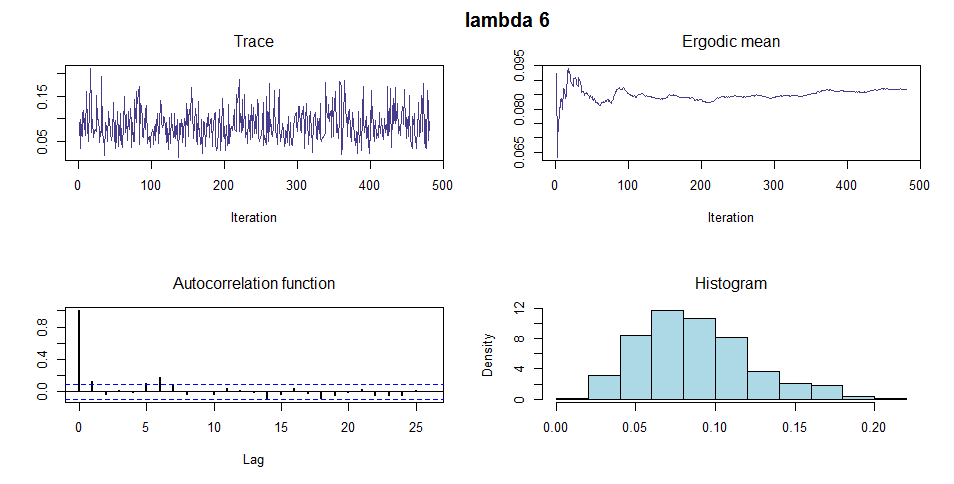
\includegraphics[width=\textwidth]{G23.png}
  \caption{Gamma Example 2 - Diagnosis for $\lambda_6$}
  \label{fig:G2a}
\end{figure}

\subsubsection{Example 3. Varying c through a distribution. Unitary length intervals}

As we reviewed, we can learn about the $\{c_k\}$ via assigning an exponential distribution with mean $\epsilon$. The estimates using $\epsilon = 1$ --\code{type.c = 3}-- and unitary length intervals --\code{type.t = 2}-- are shown in Figure \ref{fig:G3}. We can compare the hazard function with the previous example, where $c$ was fixed, and observe that because of the variability given to $c$, the change on the estimated values between two contiguous intervals are greater in this example. The survival function echoes the shape of the Kaplan-Meier with higher decrease rates. 

Comparing this example with Example 6 --Figure \ref{fig:G6}--, as with the previous example, the main difference is given by the partition of the time axis. This affects the estimates as we will note later.

\begin{knitrout}
\definecolor{shadecolor}{rgb}{0.969, 0.969, 0.969}\color{fgcolor}\begin{kframe}
\begin{alltt}
\hlstd{ExG3} \hlkwb{<-} \hlkwd{GaMRes}\hlstd{(times, delta,} \hlkwc{type.t} \hlstd{=} \hlnum{2}\hlstd{,} \hlkwc{K} \hlstd{=} \hlnum{35}\hlstd{,} \hlkwc{type.c} \hlstd{=} \hlnum{3}\hlstd{,} \hlkwc{epsilon} \hlstd{=} \hlnum{1}\hlstd{,}
               \hlkwc{iterations} \hlstd{=} \hlnum{3000}\hlstd{)}
\hlkwd{GaPloth}\hlstd{(ExG3)}
\end{alltt}
\end{kframe}
\end{knitrout}

\begin{figure}
  \centering
  \begin{subfigure}[a]{\textwidth}\centering
    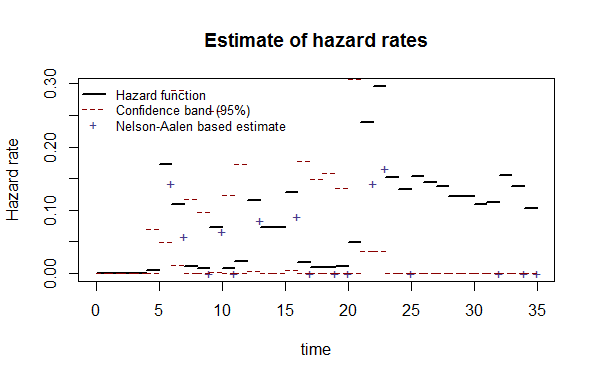
\includegraphics[width=\textwidth]{G31.png}
    \caption{Hazard rates}
  \end{subfigure}
  \begin{subfigure}[b]{\textwidth}\centering
    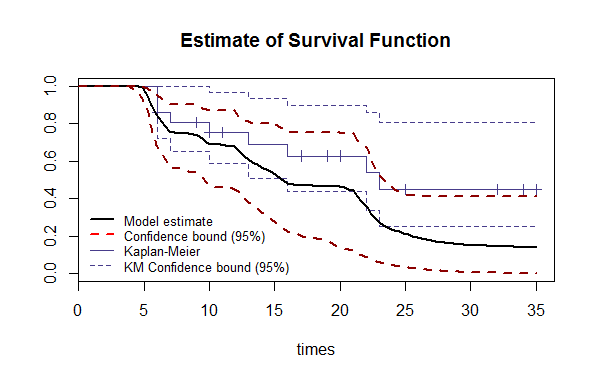
\includegraphics[width=\textwidth]{G32.png}
    \caption{Survival function}
  \end{subfigure}
  \caption{Gamma Example 3 - Varying $c$ through a distribution $c_k\sim Ga(1,\epsilon = 1$). Unitary length intervals}
  \label{fig:G3}
\end{figure}

\subsubsection{Example 4. Using a hierarchical model to estimate c. Unitary intervals}

Previous example can be extended with a hierarchical model, assigning a distribution to $\epsilon ~ \sim Ga(a_0,b_0)$ with $a_0=b_0=0.01$. In order to set up the model we should set \code{type.c = 4}. The result displayed on Figure \ref{fig:G4} is a soft hazard function and a survival function that decreases faster than the Kaplan-Meier estimate.

\begin{knitrout}
\definecolor{shadecolor}{rgb}{0.969, 0.969, 0.969}\color{fgcolor}\begin{kframe}
\begin{alltt}
\hlstd{ExG4} \hlkwb{<-} \hlkwd{GaMRes}\hlstd{(times, delta,} \hlkwc{type.t} \hlstd{=} \hlnum{2}\hlstd{,} \hlkwc{K} \hlstd{=} \hlnum{35}\hlstd{,} \hlkwc{type.c} \hlstd{=} \hlnum{4}\hlstd{,}
               \hlkwc{iterations} \hlstd{=} \hlnum{3000}\hlstd{)}
\hlkwd{GaPloth}\hlstd{(ExG4)}
\end{alltt}
\end{kframe}
\end{knitrout}

\begin{figure}
  \centering
  \begin{subfigure}[a]{\textwidth}\centering
    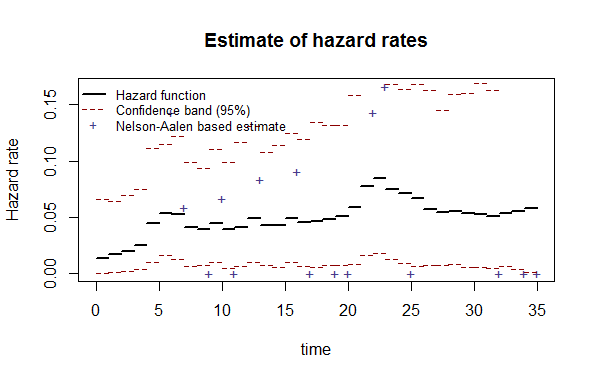
\includegraphics[width=\textwidth]{G41.png}
    \caption{Hazard rates}
  \end{subfigure}
  \begin{subfigure}[b]{\textwidth}\centering
    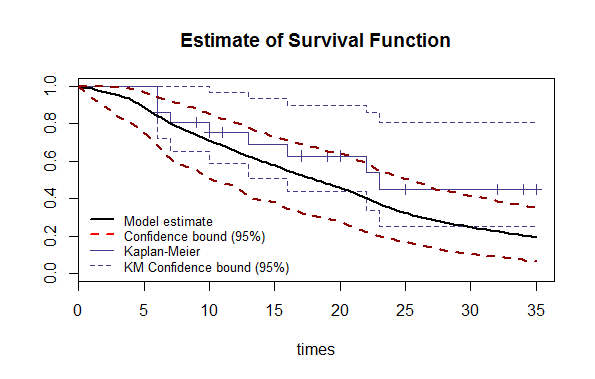
\includegraphics[width=\textwidth]{G42.png}
    \caption{Survival function}
  \end{subfigure}
  \caption{Gamma Example 4 - Using a hierarchical model to estimate $c$. Unitary intervals}
  \label{fig:G4}
\end{figure}

\subsubsection{Example 5. Introducing dependence through c. Equally dense intervals}

This example illustrates the same concept as Example 2 --how $c$ introduces dependence--, but with a different partition of the time axis. To get this partition we set \code{type.t = 1}. Figure \ref{fig:G5} shows that the survival function is close to the Kaplan-Meier estimate. The fact that it gets closer to the K-M estimates does not makes it a better estimate, we only could say that this partition yields, in average, a smaller hazard rate than the Example 2 built with a unitary length partition.

\begin{knitrout}
\definecolor{shadecolor}{rgb}{0.969, 0.969, 0.969}\color{fgcolor}\begin{kframe}
\begin{alltt}
\hlstd{ExG5} \hlkwb{<-} \hlkwd{GaMRes}\hlstd{(times, delta,} \hlkwc{type.t} \hlstd{=} \hlnum{1}\hlstd{,} \hlkwc{K} \hlstd{=} \hlnum{8}\hlstd{,} \hlkwc{type.c} \hlstd{=} \hlnum{2}\hlstd{,}
               \hlkwc{c.r} \hlstd{=} \hlkwd{rep}\hlstd{(}\hlnum{50}\hlstd{,} \hlnum{7}\hlstd{),} \hlkwc{iterations} \hlstd{=} \hlnum{3000}\hlstd{)}
\hlkwd{GaPloth}\hlstd{(ExG5)}
\end{alltt}
\end{kframe}
\end{knitrout}

\begin{figure}
  \centering
  \begin{subfigure}[a]{\textwidth}\centering
    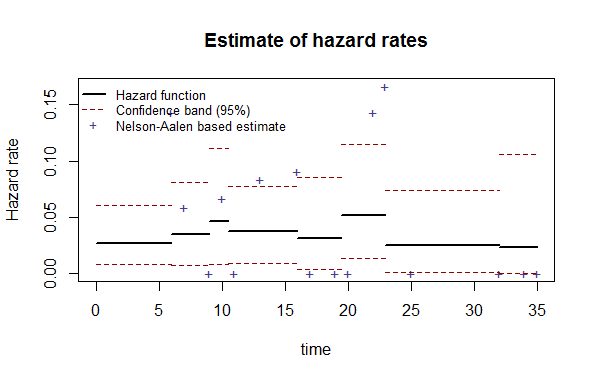
\includegraphics[width=\textwidth]{G51.png}
    \caption{Hazard rates}
  \end{subfigure}
  \begin{subfigure}[b]{\textwidth}\centering
    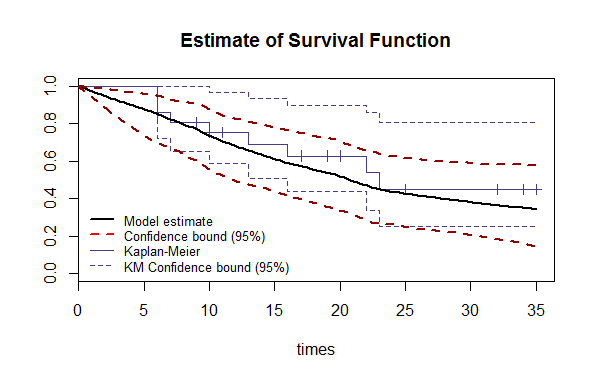
\includegraphics[width=\textwidth]{G52.png}
    \caption{Survival function}
  \end{subfigure}
  \caption{Gamma Example 5 - Introducing dependence through $c$ ($c_k=50, \forall k$). Equally dense intervals}
  \label{fig:G5}
\end{figure}

\subsubsection{Example 6. Varying c through a distribution. Equally dense intervals}

We can compare this example on Figure \ref{fig:G6} with Example 3 --Figure \ref{fig:G3}--. We use less intervals, so the survival function is smoother. Our estimate decreases faster than the Kaplan-Meier estimate. 

\begin{knitrout}
\definecolor{shadecolor}{rgb}{0.969, 0.969, 0.969}\color{fgcolor}\begin{kframe}
\begin{alltt}
\hlstd{ExG6} \hlkwb{<-} \hlkwd{GaMRes}\hlstd{(times, delta,} \hlkwc{type.t} \hlstd{=} \hlnum{1}\hlstd{,} \hlkwc{K} \hlstd{=} \hlnum{8}\hlstd{,} \hlkwc{type.c} \hlstd{=} \hlnum{3}\hlstd{,}
               \hlkwc{iterations}\hlstd{=}\hlnum{3000}\hlstd{)}
\hlkwd{GaPloth}\hlstd{(ExG6)}
\end{alltt}
\end{kframe}
\end{knitrout}

\begin{figure}
  \centering
  \begin{subfigure}[a]{\textwidth}\centering
    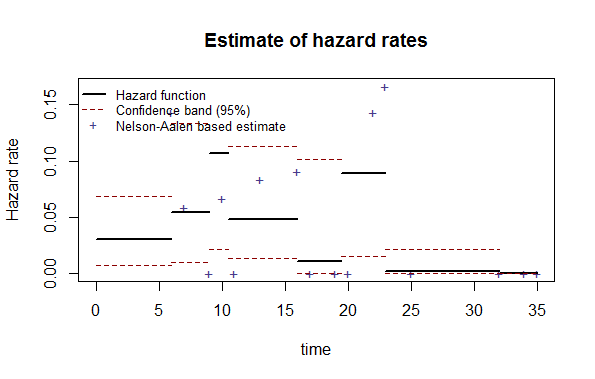
\includegraphics[width=\textwidth]{G61.png}
    \caption{Hazard rates}
  \end{subfigure}
  \begin{subfigure}[b]{\textwidth}\centering
    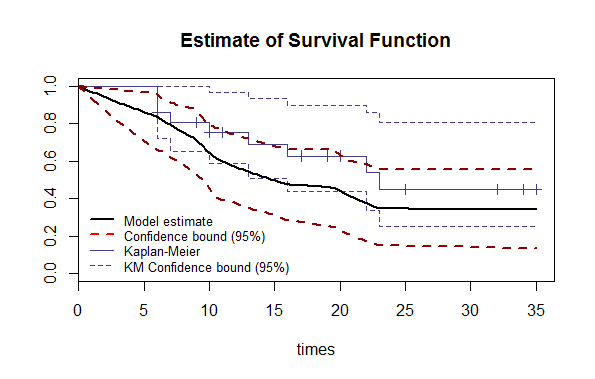
\includegraphics[width=\textwidth]{G62.png}
    \caption{Survival function}
  \end{subfigure}
  \caption{Gamma Example 6 - Varying $c$ through a distribution $c_k\sim Ga(1,\epsilon = 1$). Equally dense intervals}
  \label{fig:G6}
\end{figure}

\subsubsection{Example 7. Using a hierarchical model to estimate c. Equally dense intervals}

The survival curve for this particular example results in a smoothed version of the Kaplan-Meier estimate (Figure \ref{fig:G7}). As with previous examples, it can be compared with the unitary partition example (see Example 4, Figure \ref{fig:G4}). 

\begin{knitrout}
\definecolor{shadecolor}{rgb}{0.969, 0.969, 0.969}\color{fgcolor}\begin{kframe}
\begin{alltt}
\hlstd{ExG7} \hlkwb{<-} \hlkwd{GaMRes}\hlstd{(times, delta,} \hlkwc{type.t} \hlstd{=} \hlnum{1}\hlstd{,} \hlkwc{K} \hlstd{=} \hlnum{8}\hlstd{,} \hlkwc{type.c} \hlstd{=} \hlnum{4}\hlstd{,}
               \hlkwc{iterations} \hlstd{=} \hlnum{3000}\hlstd{)}
\hlkwd{GaPloth}\hlstd{(ExG7)}
\end{alltt}
\end{kframe}
\end{knitrout}

\begin{figure}
  \centering
  \begin{subfigure}[a]{\textwidth}\centering
    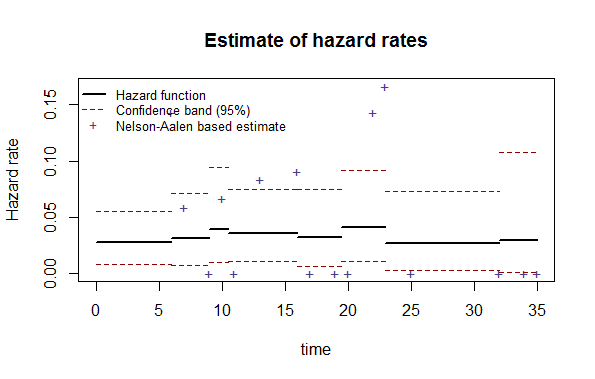
\includegraphics[width=\textwidth]{G71.png}
    \caption{Hazard rates}
  \end{subfigure}
  \begin{subfigure}[b]{\textwidth}\centering
    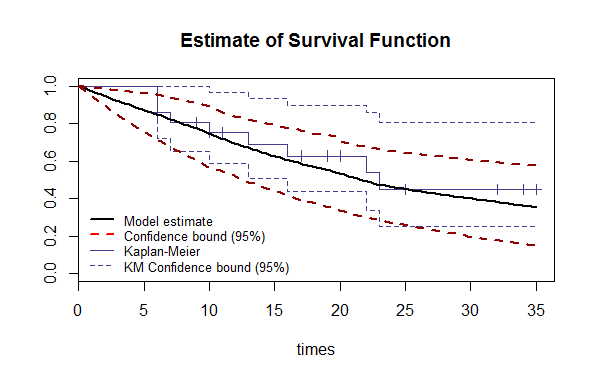
\includegraphics[width=\textwidth]{G72.png}
    \caption{Survival function}
  \end{subfigure}
  \caption{Gamma Example 7 - Using a hierarchical model to estimate $c$. Equally dense intervals}
  \label{fig:G7}
\end{figure}

%\clearpage

\subsection{Beta model examples}
For this model, we use survival data on 26 psychiatric inpatients admitted to the University of Iowa hospitals during the years 1935-1948. This sample is part of a larger study of psychiatric inpatients discussed by Tsuang and Woolson (1977). We take the \code{"time"} column as the observed times vector --\code{times}-- and the \code{"death"} column as the censoring status vector --\code{delta}--:

\begin{knitrout}
\definecolor{shadecolor}{rgb}{0.969, 0.969, 0.969}\color{fgcolor}\begin{kframe}
\begin{alltt}
\hlkwd{data}\hlstd{(psych)}
\hlstd{times} \hlkwb{<-} \hlstd{psych}\hlopt{$}\hlstd{time}
\hlstd{delta} \hlkwb{<-} \hlstd{psych}\hlopt{$}\hlstd{death}
\end{alltt}
\end{kframe}
\end{knitrout}

\subsubsection{Example 1. Independence case}

As with the Gamma Example, we obtain the Nelson-Aalen and Kaplan-Meier estimators by defining $c_k$ as a null vector through fixing \code{type.c = 1} --see Figure \ref{fig:B1}-- The conclusion does not change: the independence case of our model results on the N-A and K-M estimators.

\begin{knitrout}
\definecolor{shadecolor}{rgb}{0.969, 0.969, 0.969}\color{fgcolor}\begin{kframe}
\begin{alltt}
\hlstd{ExB1} \hlkwb{<-} \hlkwd{BeMRes}\hlstd{(times, delta,} \hlkwc{type.c} \hlstd{=} \hlnum{1}\hlstd{,} \hlkwc{iterations} \hlstd{=} \hlnum{3000}\hlstd{)}
\hlkwd{BePloth}\hlstd{(ExB1,} \hlkwc{confint} \hlstd{=} \hlnum{FALSE}\hlstd{)}
\end{alltt}
\end{kframe}
\end{knitrout}

\begin{figure}
  \centering
  \begin{subfigure}[a]{\textwidth}\centering
    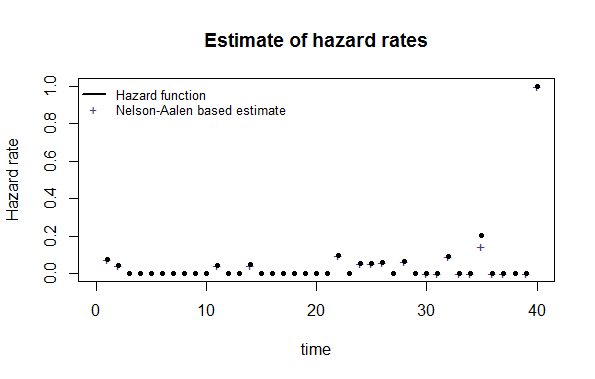
\includegraphics[width=\textwidth]{B11.png}
    \caption{Hazard rates}
  \end{subfigure}
  \begin{subfigure}[b]{\textwidth}\centering
    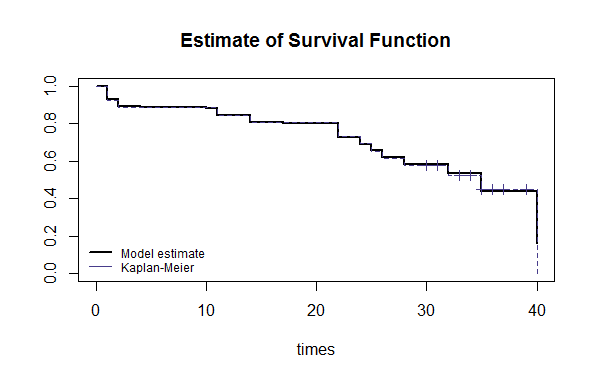
\includegraphics[width=\textwidth]{B12.png}
    \caption{Survival function}
  \end{subfigure}
  \caption{Beta Example 1 - Independence case}
  \label{fig:B1}
\end{figure}
 
\subsubsection{Example 2. Introducing dependence through c}

The influence of $c$ --or \code{c.r}-- can be also understood as a dependence parameter: the greater the value of each $c_k$, $k=0,1,2,...,K-1$, the higher the dependence between intervals $k$ and $k+1$. In this example, we fix each $c$ entry at 100. As we are defining vector $c$ with fixed values, we should fix \code{type.c = 2}. We see on Figure \ref{fig:B2} that the hazard function estimate turns smoother than on the previous example. The steps on the survival function appear to be more uniform than on the Kaplan-Meier estimate. 
 
\begin{knitrout}
\definecolor{shadecolor}{rgb}{0.969, 0.969, 0.969}\color{fgcolor}\begin{kframe}
\begin{alltt}
\hlstd{ExB2} \hlkwb{<-} \hlkwd{BeMRes}\hlstd{(times, delta,} \hlkwc{type.c} \hlstd{=} \hlnum{2}\hlstd{,} \hlkwc{c.r} \hlstd{=} \hlkwd{rep}\hlstd{(}\hlnum{100}\hlstd{,} \hlnum{39}\hlstd{),}
               \hlkwc{iterations} \hlstd{=} \hlnum{3000}\hlstd{)}
\hlkwd{BePloth}\hlstd{(ExB2)}
\end{alltt}
\end{kframe}
\end{knitrout}

\begin{figure}
  \centering
  \begin{subfigure}[a]{\textwidth}\centering
    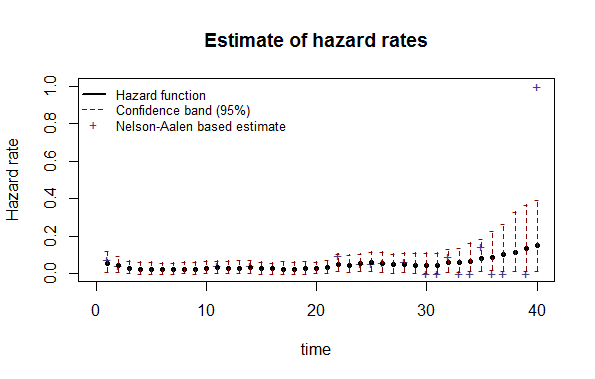
\includegraphics[width=\textwidth]{B21.png}
    \caption{Hazard rates}
  \end{subfigure}
  \begin{subfigure}[b]{\textwidth}\centering
    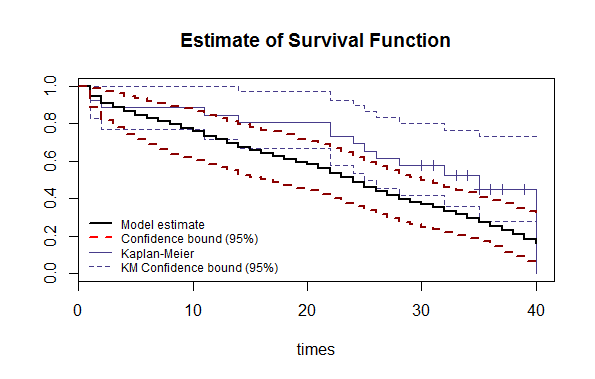
\includegraphics[width=\textwidth]{B22.png}
    \caption{Survival function}
  \end{subfigure}
  \caption{Beta Example 2 - Introducing dependence through $c$ ($c_k=100, \forall k)$}
  \label{fig:B2}
\end{figure}

Additionally, we can get further detail on the Gibbs sampler with a diagnosis of the resulting Markov chain. We can run this diagnosis for each entry from $\pi$, $u$, $c$ or $\epsilon$. In Figure \ref{fig:B2a} we show the diagnosis for $\pi_{10}$ which includes plot of the trace, the ergodic mean, the ACF function and the histogram of the chain.

\begin{knitrout}
\definecolor{shadecolor}{rgb}{0.969, 0.969, 0.969}\color{fgcolor}\begin{kframe}
\begin{alltt}
\hlkwd{BePlotDiag}\hlstd{(ExB2,} \hlkwc{variable} \hlstd{=} \hlstr{"Pi"}\hlstd{,} \hlkwc{pos} \hlstd{=} \hlnum{6}\hlstd{)}
\end{alltt}
\end{kframe}
\end{knitrout}

\begin{figure}
  \centering
  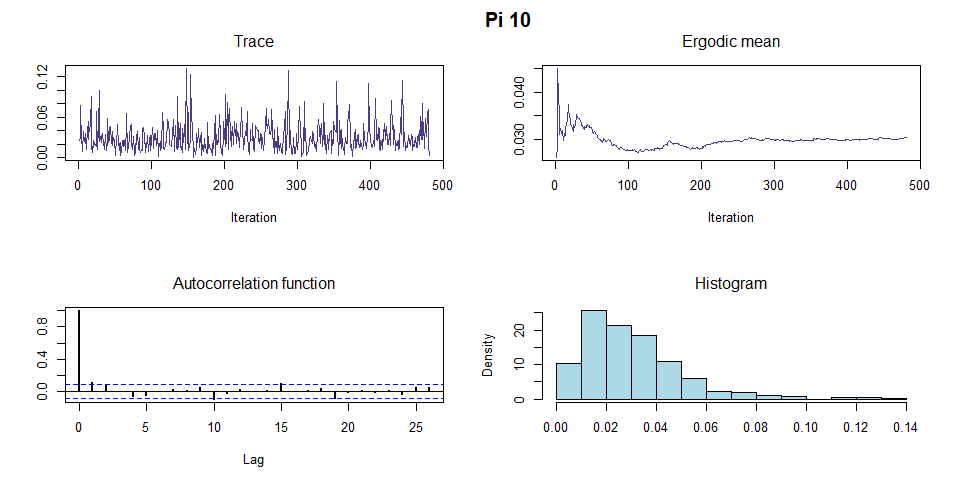
\includegraphics[width=\textwidth]{B23.png}
  \caption{Beta Example 2 - Diagnosis for $\pi_{10}$}
  \label{fig:B2a}
\end{figure}

\subsubsection{Example 3. Varying c through a distribution}

As with the gamma model, we can learn about the $\{c_k\}$ via assigning an exponential distribution with mean $\epsilon$. The estimates using $\epsilon = 1$ and unitary length intervals are shown on Figure \ref{fig:B3}. Note that the confidence intervals have widen: it is a signal that we have introduced variability to the model --because of the distribution assigned to $c$--.
 
\begin{knitrout}
\definecolor{shadecolor}{rgb}{0.969, 0.969, 0.969}\color{fgcolor}\begin{kframe}
\begin{alltt}
\hlstd{ExB3} \hlkwb{<-} \hlkwd{BeMRes}\hlstd{(times, delta,} \hlkwc{type.c} \hlstd{=} \hlnum{3}\hlstd{,} \hlkwc{epsilon} \hlstd{=} \hlnum{1}\hlstd{,} \hlkwc{iterations} \hlstd{=} \hlnum{3000}\hlstd{)}
\hlkwd{BePloth}\hlstd{(ExB3)}
\end{alltt}
\end{kframe}
\end{knitrout}

\begin{figure}
  \centering
  \begin{subfigure}[a]{\textwidth}\centering
    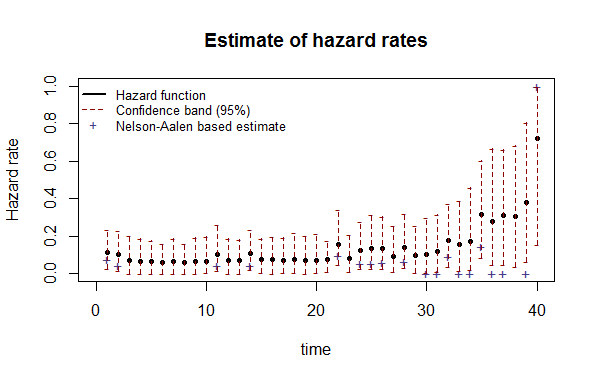
\includegraphics[width=\textwidth]{B31.png}
    \caption{Hazard rates}
  \end{subfigure}
  \begin{subfigure}[b]{\textwidth}\centering
    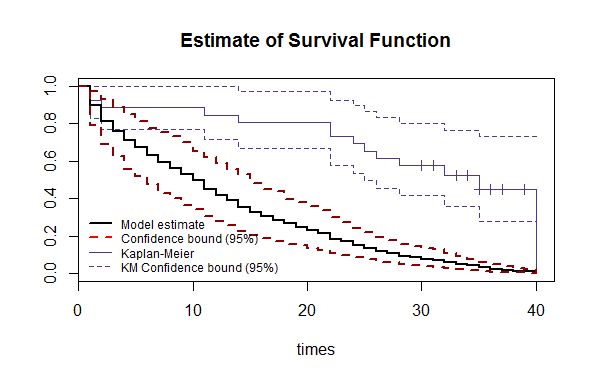
\includegraphics[width=\textwidth]{B32.png}
    \caption{Survival function}
  \end{subfigure}
  \caption{Beta Example 3 - Varying $c$ through a distribution $c_k\sim Ga(1,\epsilon = 1)$}
  \label{fig:B3}
\end{figure}

\subsubsection{Example 4. Using a hierarchical model to estimate c}

The previous example can be extended with a hierarchical model, assigning a distribution to $\epsilon ~ \sim Ga(a_0,b_0)$, with $a_0=b_0=0.01$. In order to set up the model we should set \code{type.c = 4}. The result displayed on Figure \ref{fig:B4} is a soft hazard function and a survival function that decreases faster than the Kaplan-Meier estimate.

\begin{knitrout}
\definecolor{shadecolor}{rgb}{0.969, 0.969, 0.969}\color{fgcolor}\begin{kframe}
\begin{alltt}
\hlstd{ExB4} \hlkwb{<-} \hlkwd{BeMRes}\hlstd{(times, delta,} \hlkwc{type.c} \hlstd{=} \hlnum{4}\hlstd{,} \hlkwc{iterations} \hlstd{=} \hlnum{3000}\hlstd{)}
\hlkwd{BePloth}\hlstd{(ExB4)}
\end{alltt}
\end{kframe}
\end{knitrout}

\begin{figure}
  \centering
  \begin{subfigure}[a]{\textwidth}\centering
    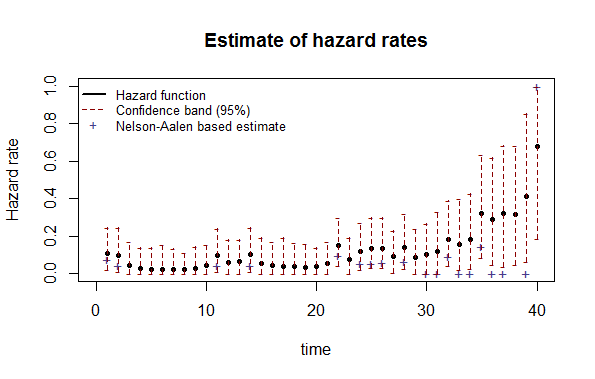
\includegraphics[width=\textwidth]{B41.png}
    \caption{Hazard rates}
  \end{subfigure}
  \begin{subfigure}[b]{\textwidth}\centering
    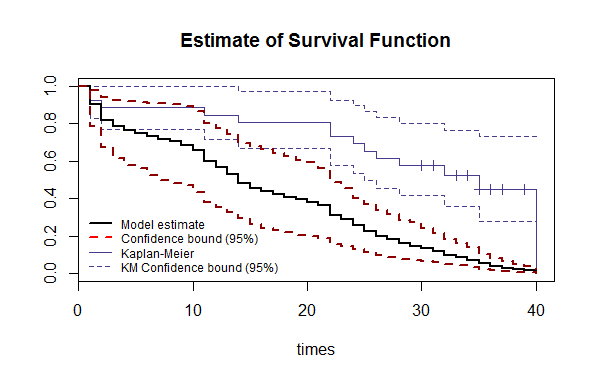
\includegraphics[width=\textwidth]{B42.png}
    \caption{Survival function}
  \end{subfigure}
  \caption{Beta Example 4 - Using a hierarchical model to estimate $c$}
  \label{fig:B4}
\end{figure}

\clearpage

\subsection{Cox-gamma model example}

In this example, we simulate the data from a Weibull model, frequently used with continuous and non negative data. The advantage of setting a model is that we know in advance the results, so we can compare the estimates with the exact values from model. The Weibull model has the probability functions:
\begin{equation*}
  h_0(t)=abt^{b-1}, S_0(t)=e^{-at^b}
\end{equation*}

We construct the proportional hazard model as:
\begin{equation*}
h_i(t_i|Z_i)=h_0(t)e^{\theta 'Z_i}bt^{b-1}, S_i(t_i|Z_i)=exp\left\{-H_0(t_i)e^{\theta 'Z_i}\right\}
\end{equation*}

Note that this Weibull proportional hazard model is also another Weibull model with parameters ($a_i^*=ae^{\theta 'Z_i},b$). Based on the previous densities and on fixed parameters $a,b,\theta_1$ and $\theta_2$ -these last two covariates are simulated from uniform distributions on the interval (0,1)-, we simulate $n$ observations. We gather the results of the model in a table --see Table \ref{cuad:weibull}--. $t_i|Z_i \sim Weibull(a_i^*, b)$ and $Z_i = (Z_{i1},Z_{i2})$ are the explanatory variables; $c_i$, the censoring time; $\delta_i$, censoring indicator, and $min\{t_i,c_i\}$ represents \emph{observed} values deeming censorship time.

\begin{table}
  \centering
	\begin{tabular}{|c| c| c| c| c| c| c|}
		\hline
		i & $t_i$ &$Z_{i1}\sim U(0,1)$ & $Z_{i2}\sim U(0,1)$   & $c_i\sim Exp(1)$ & $\delta_i=I(t_i>c_i)$ & $min\{t_i,c_i\}$ \\
		\hline
 		1 &$t_1$ & $Z_{11}$ & $Z_{12}$ &  $c_1$ & $\delta_1$ & $min\{t_1,c_1\}$  \\
 		2 &$t_2$ & $Z_{21}$ & $Z_{22}$ &  $c_2$ & $\delta_2$ & $min\{t_2,c_2\}$  \\
 		$\vdots$ & $\vdots$ &$\vdots$ &$\vdots$ &$\vdots$ &$\vdots$ &$\vdots$  \\
 		$n$ &$t_n$ & $Z_{n1}$ & $Z_{n2}$ & $c_n$ & $\delta_n$ & $min\{t_n,c_n\}$  \\
  		\hline
	\end{tabular}
	\caption{Weibull simulation model}
	\label{cuad:weibull}
\end{table}

We generate a size $n=100$ sample based on the simulation model with parameters $a=$0.1, $b=1,\theta=(1,1)$ y $Z_i\sim U(0,1)$, $i=1,2$. The result is a table with $n=100$ observations.

On the other hand, we use almost every default parameter from \code{CGaMRes} excluding \code{K = 10}, \code{iterations = 3000} and \code{thpar = 10}. Theoretically, our model should estimate a constant risk function at $a\times b=0.1$. 

Below, we show the code for the Weibull model and the calls for the plots for the hazard and survival functions --command \code{CGaPloth(M)}--, the predictive distribution for an observation defined as the median of the data --\code{CGaPred(M)}--, and the plots for $\theta_1$ and $\theta_2$ --\code{PlotTheta(M)}--.

\begin{knitrout}
\definecolor{shadecolor}{rgb}{0.969, 0.969, 0.969}\color{fgcolor}\begin{kframe}
\begin{alltt}
\hlstd{SampWeibull} \hlkwb{<-} \hlkwa{function}\hlstd{(}\hlkwc{n}\hlstd{,} \hlkwc{a} \hlstd{=} \hlnum{10}\hlstd{,} \hlkwc{b} \hlstd{=} \hlnum{1}\hlstd{,} \hlkwc{beta} \hlstd{=} \hlkwd{c}\hlstd{(}\hlnum{1}\hlstd{,} \hlnum{1}\hlstd{)) \{}
  \hlstd{M} \hlkwb{<-} \hlkwd{matrix}\hlstd{(}\hlnum{0}\hlstd{,} \hlkwc{ncol} \hlstd{=} \hlnum{7}\hlstd{,} \hlkwc{nrow} \hlstd{= n)}
  \hlkwa{for}\hlstd{(i} \hlkwa{in} \hlnum{1}\hlopt{:}\hlstd{n)\{}
    \hlstd{M[i,} \hlnum{1}\hlstd{]} \hlkwb{<-} \hlstd{i}
    \hlstd{M[i,} \hlnum{2}\hlstd{]} \hlkwb{<-} \hlstd{x1} \hlkwb{<-} \hlkwd{runif}\hlstd{(}\hlnum{1}\hlstd{)}
    \hlstd{M[i,} \hlnum{3}\hlstd{]} \hlkwb{<-} \hlstd{x2} \hlkwb{<-} \hlkwd{runif}\hlstd{(}\hlnum{1}\hlstd{)}
    \hlstd{M[i,} \hlnum{4}\hlstd{]} \hlkwb{<-} \hlkwd{rweibull}\hlstd{(}\hlnum{1}\hlstd{,} \hlkwc{shape} \hlstd{= b,}
                        \hlkwc{scale} \hlstd{=} \hlnum{1} \hlopt{/} \hlstd{(a} \hlopt{*} \hlkwd{exp}\hlstd{(}\hlkwd{cbind}\hlstd{(x1, x2)} \hlopt \hlstd{beta)))}
    \hlstd{M[i,} \hlnum{5}\hlstd{]} \hlkwb{<-} \hlkwd{rexp}\hlstd{(}\hlnum{1}\hlstd{)}
    \hlstd{M[i,} \hlnum{6}\hlstd{]} \hlkwb{<-} \hlstd{M[i,} \hlnum{4}\hlstd{]} \hlopt{>} \hlstd{M[i,} \hlnum{5}\hlstd{]}
    \hlstd{M[i,} \hlnum{7}\hlstd{]} \hlkwb{<-} \hlkwd{min}\hlstd{(M[i,} \hlnum{4}\hlstd{], M[i,} \hlnum{5}\hlstd{])}
  \hlstd{\}}
  \hlkwd{colnames}\hlstd{(M)} \hlkwb{<-} \hlkwd{c}\hlstd{(}\hlstr{"i"}\hlstd{,} \hlstr{"x_i1"}\hlstd{,} \hlstr{"x_i2"}\hlstd{,} \hlstr{"t_i"}\hlstd{,} \hlstr{"c_i"}\hlstd{,} \hlstr{"delta"}\hlstd{,}
                   \hlstr{"min\{c_i, d_i\}"}\hlstd{)}
  \hlkwd{return}\hlstd{(M)}
\hlstd{\}}
\hlstd{dat} \hlkwb{<-} \hlkwd{SampWeibull}\hlstd{(}\hlnum{100}\hlstd{,} \hlnum{0.1}\hlstd{,} \hlnum{1}\hlstd{,} \hlkwd{c}\hlstd{(}\hlnum{1}\hlstd{,} \hlnum{1}\hlstd{))}
\hlstd{dat} \hlkwb{<-} \hlkwd{cbind}\hlstd{(dat[,} \hlkwd{c}\hlstd{(}\hlnum{4}\hlstd{,} \hlnum{6}\hlstd{)], dat[,} \hlkwd{c}\hlstd{(}\hlnum{2}\hlstd{,} \hlnum{3}\hlstd{)])}
\hlstd{CG} \hlkwb{<-} \hlkwd{CGaMRes}\hlstd{(dat,} \hlkwc{K} \hlstd{=} \hlnum{10}\hlstd{,} \hlkwc{iterations} \hlstd{=} \hlnum{3000}\hlstd{,} \hlkwc{thpar} \hlstd{=} \hlnum{10}\hlstd{)}
\hlkwd{CGaPloth}\hlstd{(CG)}
\hlkwd{PlotTheta}\hlstd{(CG)}
\hlkwd{CGaPred}\hlstd{(CG)}
\end{alltt}
\end{kframe}
\end{knitrout}

Because of the way we built the model, we can compare against theoretical results on the Weibull model. In Figure \ref{fig:CG1} we see that the hazard rate estimate is practically the same from t = 8 to t = 37. The estimate for the survival functions gets very close to the real value. Plots and histograms for $\theta$ from Figure \ref{fig:CG2} show estimated values for the regression coefficients $(\theta_1,\theta_2)$ and they are consistently near to 1. Finally, the plots from Figure \ref{fig:CG3} show the hazard rate estimate over a equally dense partition for a future individual where its explanatory variable is equal to the median of the observations --$x_F$--. Note that the effect over the hazard function is given by the product of the baseline hazard function and $\exp\{x_F'\theta\}$.
 
\begin{figure}
  \centering
  \begin{subfigure}[b]{\textwidth}\centering
    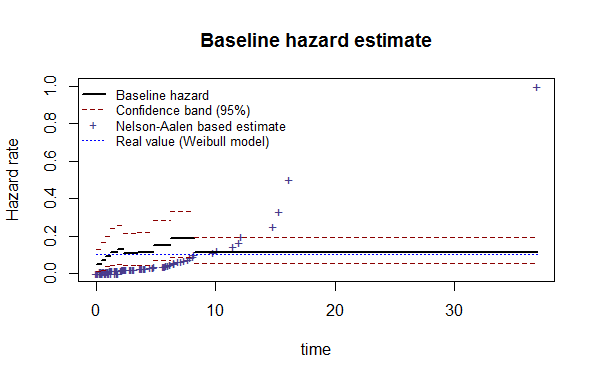
\includegraphics[width=\textwidth]{CG1.png}
    \caption{Hazard rate estimate}
  \end{subfigure}
  \begin{subfigure}[b]{\textwidth}\centering
    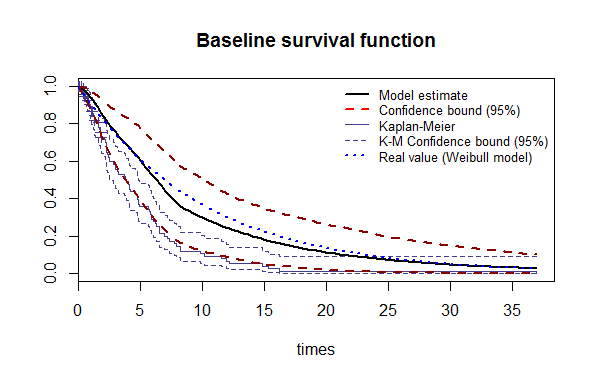
\includegraphics[width=\textwidth]{CG2.png}
    \caption{Survival function estimate}
  \end{subfigure}
  \caption{Cox-gamma example}
  \label{fig:CG1}
\end{figure}

\begin{figure}
  \centering
  \begin{subfigure}[b]{\textwidth}\centering
    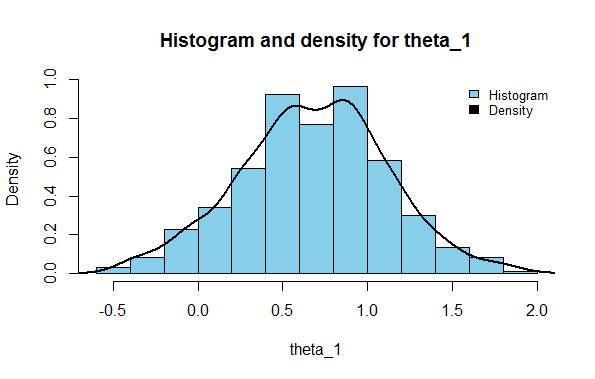
\includegraphics[width=\textwidth]{CG3.png}
    \caption{$\theta_1$ estimate}
  \end{subfigure}
  \begin{subfigure}[b]{\textwidth}\centering
    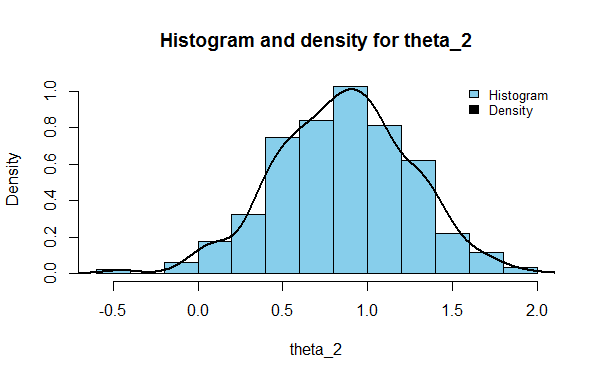
\includegraphics[width=\textwidth]{CG4.png}
    \caption{$\theta_2$ estimate}
  \end{subfigure}
  \caption{$\theta$ estimate on the Cox-gamma example}
  \label{fig:CG2}
\end{figure}

\begin{figure}
  \centering
  \begin{subfigure}{\textwidth}
    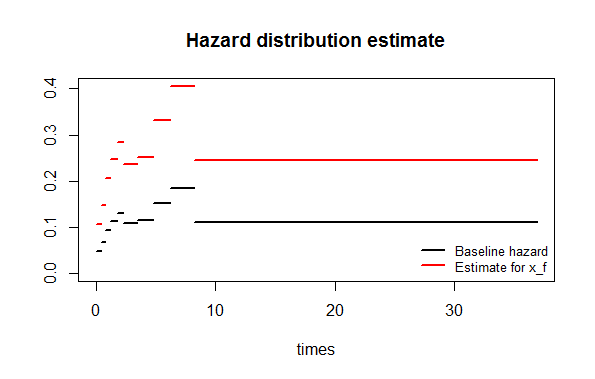
\includegraphics[width=\textwidth]{CG5.png}
  \end{subfigure}
  \caption{Hazard rate estimate for the median on the Cox-gamma example}
  \label{fig:CG3}
\end{figure}

\pagebreak

\section{References}

\begin{itemize}
  \item{ \textsc{Freireich. E.J., et al.}, Estimation of Exponential Survival Probabilities with Concomitant Information, \textit{Biometrics}, {\bf 21}, pages: 826-838, 1965.}
  \item{ \textsc{Gehan, E.A.}, A generalized Wilcoxon test for comparing arbitrarily single-censored samples, \textit{Biometrika}, {\bf 52}, pages: 687-696, 1965.}
  \item{ \textsc{Hjort, N.L.}, Nonparametric Bayes estimators based on beta processes in models for life history data, \textit{Annals of Statistics}, {\bf 18}, p'ags: 1259-1294, 1990.}
  \item{\textsc{Kaplan, E.L.} y \textsc{Meier, P.} Nonparametric estimation from incomplete observations, \textit{Journal of the American Statistical Association} {\bf 53}. 282, p'ags: 457-481, 1958.}
    \item{\textsc{Klein. J.P.} y \textsc{Moeschberger, M.L.} Survival analysis: techniques for censored and truncated data, Springer Science \& Business Media, 2003.}
  \item{ \textsc{Nieto-Barajas, L.E.} \& \textsc{Walker, S.G.}, Markov beta and gamma processes for modelling hazard rates, \textit{Scandinavian Journal of Statistics} no. {\bf 29}, pages 413-424, 2002.}
  \item{ \textsc{Nieto-Barajas, L.E.}, Discrete time Markov gamma processes and time dependent covariates  in survival analysis, \textit{Bulletin of the International Statistical Institute 54th Session}, 2003.}
  \item{ \textsc{Tsuang, M.T. and Woolson}, R.F. Mortality in Patients with Schizophrenia, Mania and Depression, \textit{British Journal of Psychiatry}, {\bf 130}, pages 162-166, 1977.}
  \item{ \textsc{Walker, S.G.} y \textsc{Mallick, B.K.}, Hierarchical generalized linear models and frailty models with Bayesian nonparametric mixing, \textit{Journal of the Royal Statistical Society}, Series B {\bf 59}, p'ags: 845-860, 1997.}
    \item{ \textsc{Woolson, R.F.}, Rank Tests and a One-Sample Log Rank Test for Comparing Observed Survival Data to a Standard Population, \textit{Biometrics}, {\bf 37}, pages: 687-696, 1981.}
\end{itemize}

\end{document}
